% Template for PLoS
% Version 1.0 January 2009
%
% To compile to pdf, run:
% latex plos.template
% bibtex plos.template
% latex plos.template
% latex plos.template
% dvipdf plos.template

\documentclass[10pt]{article}

% amsmath package, useful for mathematical formulas
\usepackage{amsmath}
% amssymb package, useful for mathematical symbols
\usepackage{amssymb}

% graphicx package, useful for including eps and pdf graphics
% include graphics with the command \includegraphics
\usepackage{graphicx}

% cite package, to clean up citations in the main text. Do not remove.
\usepackage{cite}

\usepackage{color} 

% Use doublespacing - comment out for single spacing
%\usepackage{setspace} 
%\doublespacing

\newcommand{\argmin}{\operatornamewithlimits{argmin}}

% Text layout
\topmargin 0.0cm
\oddsidemargin 0.5cm
\evensidemargin 0.5cm
\textwidth 16cm 
\textheight 21cm

% Bold the 'Figure #' in the caption and separate it with a period
% Captions will be left justified
\usepackage[labelfont=bf,labelsep=period,justification=raggedright]{caption}

% Use the PLoS provided bibtex style
\bibliographystyle{plos2009}

% Remove brackets from numbering in List of References
\makeatletter
\renewcommand{\@biblabel}[1]{\quad#1.}
\makeatother


% Leave date blank
\date{}

\pagestyle{myheadings}
%% ** EDIT HERE **


%% ** EDIT HERE **
%% PLEASE INCLUDE ALL MACROS BELOW

%% END MACROS SECTION

\begin{document}

% Title must be 150 characters or less
\begin{flushleft}
{\Large
\textbf{Metagenome phylogeny for the 1\%}
}
% Insert Author names, affiliations and corresponding author email.
\\
Person A$^{1}$, 
Person B$^{1,2,3}$, 
Person C$^{1,\ast}$
\\
\bf{1} Genome Center, University of California-Davis, California, United States of America
\\
\bf{2} Department of Evolution and Ecology, University of California-Davis, California, United States of America
\\
\bf{3} Department. of Medical Microbiology and Immunology, University of California-Davis, California, United States of America
\\
$\ast$ E-mail: aarondarling@ucdavis.edu
\end{flushleft}

% Please keep the abstract between 250 and 300 words
\section*{Abstract}
blahdeeblah, blah blah
% Please keep the Author Summary between 150 and 200 words
% Use first person. PLoS ONE authors please skip this step. 
% Author Summary not valid for PLoS ONE submissions.   
\section*{Author Summary}

\section*{Introduction}

The emerging practice of metagenomics has for the first time offered a glimpse of the genetic structure of uncultured microbial communities.
In its current form however, metagenomics destroys some of the most valuable information present in a sample: genetic linkage.
In nearly all metagenomic sample processing methods, cells from the microbial community are lysed together to obtain the DNA.
This practice causes DNA from many different cells to mix together, so that the cellular compartmentalization of individual genotypes is lost.
Long chromosome-scale DNA fragments are then typically broken by mechanical or enzymatic means into fragments small enough for processing with current sequencing chemistries. 
The resulting sequenced fragments are usually less than 1Kbp (though sometimes 10-20kbp). 
The shearing further destroys genetic linkage information, because information on how the short fragments were arranged into chromosome-scale molecules is lost.

Improved sample-processing workflows might preserve the genetic linkage information of a microbial community through the sequencing process.
High throughput single-cell genomics (e.g. applied to thousands of cells) offers an alternative to the standard metagenomics workflow that preserves information about the compartmentalization of genetic material into cells. 
However, single-cell genomics currently presents its own challenges associated with isolating individual cells from certain types of samples and amplifying the {DNA} from a single cell to attain the minimum quantity required for sequencing. 
Furthermore, single-cell genomics has extensive equipment requirements and is highly sensitive to contamination by foreign DNA, requiring rigorous laboratory and reagent decontamination.

Given the current limitations of metagenomics, practitioners resort to computational methods to reconstruct the genetic architecture of a microbial community after sequencing.
Computational methods have demonstrated promise for metagenomic analysis and a wide range of approaches have been explored.
Metagenome linkage analysis usually addresses one or more of the following problems:
\begin{itemize}
\item Taxonomic classification of sequences
\item Community structure and organism relative abundance estimation
\item Assigning sequences to bins that correspond to some meaningful group (Binning)
\end{itemize}
Each of these problems are inter-related and many methods address two or more of these at once.
\textit{Question: should we define each of these problems?}

Molecular evolution, the joint processes of DNA replication with mutation and natural selection acting on those mutations, provides the primary signal for most read classification methods.
As species diverge, differences such as nucleotide substitutions, insertions, deletions, and genomic rearrangements accumulate in their genomes, and these differences can be leveraged to infer a sequence's origin in a mixed metagenomic sample.

In the present manuscript, we introduce a new method for reconstructing the genetic architecture of a metagenomic sample and for comparison of community structure among multiple related samples.
The new method leverages explicitly phylogenetic models of molecular evolution. 
We contribute an open-source implementation of the method that has been engineered for ease-of-use on 64-bit Linux and Mac platforms.
Finally, we compare the features of the new method to some related methods to provide readers with insight into when use of the new method is and is not appropriate.


\subsection*{Previous work}
Metagenomics is a burgeoning field, we focus here on shotgun metagenome sequencing approaches and 
do not discuss analysis methods for other aspects of microbial ecology such as amplicon sequencing data such as QIIME and others. 
\subsubsection*{Whole metagenome binning}
- composition classifiers
  - TACOA~\cite{Diaz2009}, PhyloPythia 1 \& 2\cite{Patil2011},Eu-Detect\cite{Mohammed2011},ProViDE~\cite{Ghosh2011}
- identity/homology classifiers
  - MEGAN~\cite{Huson2007}, SORT-Items~\cite{Haque2009}, NBC~\cite{Rosen2011}, MTR~\cite{Gori2011}, others
\subsubsection*{Estimating community composition from metagenomes}
      - AMPHORA\cite{WuEisen2008}, MLTreeMap\cite{Stark2010}, others?
      - MetaPHlan (under review)
      - EMIRGE\cite{Miller2011}
\subsubsection*{Amplicon analysis methods}
Many community composition methods rely on amplicon sequencing. 
The analysis methods are different to metagenomics in many ways.
This is a very mature area with too many methods to list.

% You may title this section "Methods" or "Models". 
% "Models" is not a valid title for PLoS ONE authors. However, PLoS ONE
% authors may use "Analysis" 
\section*{Methods or Design and Implementation}

PhyloSift implements a method for analyzing microbial community structure directly from metagenome sequence data.
Figure~\ref{fig:overview} gives an overview of the analysis workflow as executed when analyzing a metagenomic sample.
The analysis can be decomposed into four stages: 1. searching input sequences for identity to a database of known reference gene families, 2. adding input sequences to a multiple alignment with reference genes, 3. placement of input sequences onto a phylogeny of reference genes, and 4. generation of taxonomic summaries. We now describe the details of each step along with our design decisions and rationale.
 

\subsection*{Detailed PhyloSift client workflow}
\subsubsection*{Sequence identity search}
This first step in a PhyloSift analysis aims to identify regions of the input sequences that may be homologous to gene families in the reference database.
Input sequences to this step can be of any length ranging from short 30nt next-generation sequence reads to fully assembled genomes.
Recognized input formats include FastA and FastQ (paired, unpaired, phred33, phred64, and/or interleaved pairing), and these can optionally be supplied as bzip2 or gzip compressed data files. 
Amino acid input sequences can also be processed.

PhyloSift uses LAST~\cite{Kiełbasa2011} and bowtie2~\cite{Langmead2009} for sequence similarity search against the reference databases.
We evaluated many possible search algorithms and implementations before finally selecting LAST and bowtie2. 
Other options we evaluated were BLAST~\cite{Altschul1997}, BLAST+~\cite{Camacho2009}, and RAPsearch2~\cite{Zhao2011}.
Given the large volume of sequence data that must be processed, a key evaluation criterion was algorithm efficiency both in CPU time and memory requirements. 
A second criterion is the ability to perform six-frame translated searches of DNA sequence against an amino acid database with the possibility to tolerate frame-shift errors in the sequence.
Among the evaluated methods, BLAST and BLAST+ were slowest (data not shown) and frameshift detection was non-functional in the version of BLAST+ we obtained from NCBI. We excluded these from futher consideration.
RAPsearch2 was much more computationally efficient than either BLAST or BLAST+, but the version we obtained could not process sequences > 1kbp and did not support frameshift detection.
 In our testing, LAST was able to process sequence data as quickly as RAPsearch2 (e.g. orders of magnitude more quickly than BLAST) and supports both frameshift detection and input sequences of arbitrary length.
LAST also supports all three of the primary search types we require: DNA vs. DNA, DNA vs. AA, and AA vs. AA.
We also evaluated bowtie2, a program typically used for mapping reads to a reference genome, for the purpose of screening reads against a database of noncoding RNA sequences (currently 16S and 18S).
Relative to LAST, bowtie2 is able to identify similarity to the RNA database sequences much more quickly.
Therefore we implemented bowtie2 to search short sequences against the RNA databases and LAST for all other search types.
One minor shortcoming of LAST is that current versions do not support multithreaded parallelism.
PhyloSift implements optional process-level parallelism at this stage by spawning multiple LAST searches against the protein database.

One feature of reference gene family sequences being searched at this stage bears special mention.
During database construction (described elsewhere) a representative subset of all available sequences are selected from each gene family to be searched at this stage.
These representatives are chosen to span the phylogenetic diversity of the gene family without including closely related sequences (see Section~\ref{sec:dbupdate}).
This is important because part of LAST's fast heuristic to identify candidate regions to align involves eliminating redundant and repetitive $k$-mers from the search space~\cite{Kiełbasa2011}.
A database constructed with all sequences (and not just divergent representatives) could in principle reduce sensitivity in aligning reads to those database sequences.

The result of this stage is a set of candidate amino acid sequences that are similar to each gene family in the database and (if DNA was used as input) the corresponding untranslated DNA sequences.

\subsubsection*{Alignment to reference multiple alignment}
Prior to this stage all input sequence regions with putative homology to reference gene families have been identified and extracted.
In this stage, each candidate sequence is added to an amino acid multiple sequence alignment of the reference gene family.
If the input sequences were {DNA}, a codon multiple sequence alignment congruent to the amino acid alignment is also generated.

PhyloSift applies the \texttt{hmmalign} program from the HMMER 3.0 software~\cite{Eddy2011} to add the candidate sequences to reference multiple sequence alignments.
During construction of the PhyloSift reference database (described elsewhere) a profile-HMM is generated from a multiple alignment of the gene family reference sequences.
When processing candidate sequences, PhyloSift then uses the profile-HMM to map the input sequence to the reference multiple alignment using maximal sensitivity settings (\texttt{hmmalign --max}).
We acknowledge that application of a profile-HMM to align highly divergent sequences suffers some documented shortcomings, and this is one avenue for future improvement of PhyloSift~\cite{Loytynoja2012}.

Finally, PhyloSift concatenates the alignments of the 40 elite markers to a single multiple sequence alignment.

PhyloSift treats input sequences with similarity to non-coding RNAs differently than protein genes.
These sequences are aligned using Infernal's \texttt{cmalign} program.
Sequences longer than XXnt are aligned using the global alignment option.
Short sequences are aligned with the local alignment option using a banding threshold of $1x10^{-20}$.
This banding threshold is more sensitive than the default cmalign parameter and appears to substantially improve alignment quality for short sequences (data not shown), at the expense of much extra compute time.

\subsubsection*{Placement on a phylogenetic reference tree}

At this stage, aligned input sequences are placed onto a phylogenetic tree of the reference sequences.
PhyloSift employs pplacer~\cite{Matsen2010} for this task.
pplacer does some neat stuff.


\subsubsection*{Taxonomic summary of read placements}
At this final stage of analysis, PhyloSift summarizes the phylogenetic placements in a human-friendly format.
For each gene family, the PhyloSift database contains a gene-tree/taxonomy reconciliation encoding a pre-computed mapping of edges in the gene family phylogeny to edges in the NCBI taxonomy.
The method used to calculate these reconciliations is described in Section~\ref{sec:dbupdate}.

Input to this stage of analysis is one or more ``jplace'' format files containing an edge-labeled reference tree for a gene family along with a collection of one or more sequence placements onto that tree.
Information about each sequence's placement consists of the log-likelihood of placement at several (usually up to XX, a configurable limit) of the highest likelihood edges on the reference tree, along with the probability mass that the sequence belongs at that position of the tree, and finally the weight of the sequence. 
When analyzing unassembled reads sequence weights are typically always 1, when analyzing assembled contigs the weights may be set to a value based on estimated depth-of-coverage for that contig.

PhyloSift parses each of the jplace files and uses the gene-tree/taxonomy reconciliation to convert probability mass over read placements into a probability mass over the taxonomy, summing these masses over all reads and gene families.
Any particular edge in the gene tree may be mapped to many equally optimal locations in the taxonomy.
PhyloSift distributes the placed sequence's mass equally among all optimal locations.

Finally, PhyloSift reports the summarized taxonomy probability mass distribution in a variety of formats.

\subsubsection*{Visual presentation of taxonomic summary}

For easy visualization and exploratory data analysis, PhyloSift produces Krona plots~\cite{Ondov2011} showing taxonomic probability mass in the 40 elite gene families, and a separate krona plot showing taxonomic probability mass distribution summed across the elite families and all other families.

Figure~\ref{fig:kronaplots} provide an example of PhyloSift's krona reports.

\subsubsection*{Parallelism and stream computing}

\subsubsection*{Comparison among samples}

One of the unique aspects of PhyloSift relative to other metagenome binning methods is that the phylogenetic approach we have implemented enables direct comparison of the phylogenetic structure and relative abundance of metagenome samples without resorting to taxonomic relative abundance estimates.
Perhaps the most powerful exploratory data analysis tool for comparing community structures among samples is Edge Principal Component Analysis, or Edge PCA~\cite{Matsen2012}.
Edge PCA applies the standard dimensionality-reduction tool of PCA to a matrix where columns correspond to edges in the reference phylogeny, rows correspond to each sample, and each entry is the difference in placed sequence probability masses on either side of that edge.
When applied in this manner, the eigenvalues of each eigenvector that results from PCA correspond to weights indicating how important each edge in the reference phylogeny is for explaining the variation among samples in that dimension.
Matsen and Evans showed that these eigenvectors can be naturally visualized as thickened branches along the reference phylogeny.

PhyloSift includes the guppy program from pplacer, which in addition to Edge PCA also provides means for hierarchical clustering of multiple samples, calculation of Kantorovich-Rubenstein distances among samples, and other tools for calculating sample summary statistics such as weighted phylogenetic diversity.

\subsection*{Gene families used by PhyloSift}

The standard PhyloSift database includes a set of 40 gene families previously identified as nearly universal among bacteria and archaea and in single-copy~\cite{Wu2012}.
In other work we have demonstrated that phylogenetic trees reconstructed on individual genes in this set are generally consistent with each other~\cite{Lang2012}, suggesting that concatenating alignments of these families will yield a valid and more powerful estimate of their phylogenetic history.
During the database update process (described below), these gene families are automatically extended to include putative homologs from eukarya and some viruses with large genomes such as the Mimivirus.
Most small viral genomes lack homologs of these gene families.

In addition to the elite 40 families, the PhyloSift database also includes four additional sets of gene families:
\begin{itemize}
\item \textbf{16s and 18s ribosomal RNA genes}
\item \textbf{mitochondrial gene families}
\item \textbf{Eukaryote-specific gene families}
\item \textbf{Viral gene families}
\end{itemize}

\subsection*{PhyloSift database update workflow}\label{sec:dbupdate}
An integral component of PhyloSift is an automated means to update the gene family database with newly sequenced genomes.
Genome databases continue to grow quickly, with dozens of new genome sequences becoming available every week.
The quality of these genomes can be highly variable, ranging from low-quality drafts to nearly finished sequence.
PhyloSift's database update mechanism incorporates some basic quality control mechanisms.
\subsubsection*{Acquire new genome data}
The PhyloSift database update module maintains a local repository of all known and processed genomes.
When a new update is initiated, the database update module identifies any new genomes available in the NCBI finished, NCBI draft, NCBI WGS, and EBI viral, organelle, bacterial, archaeal, and eukaryal databases. 
\subsubsection*{Gene family search and alignment workflow on each genome}
In this stage, we run the search and alignment stages of the previously described PhyloSift client workflow for each new genome.
After this stage, the regions from each new genome that are highly similar to gene families in the database are identified, extracted, and aligned using the family's profile HMM.
A complete multiple alignment for each family is then created by adding the aligned regions from each genome to a single multiple alignment file.
Because each region has been aligned to the same profile HMM (or covarion model) and non-aligning sites in the query genome removed, generation of a new multiple alignment is a simple matter of concatenating the individual alignments.

Codon alignments are also generated for each protein-coding gene family at this stage.
\subsubsection*{Phylogenetic inference}
The next step of database update involves constructing a phylogenetic tree for each gene family.
Currently PhyloSift employs FastTree 2.1~\cite{Price2010} to generate approximate maximum likelihood trees for this task.

PhyloSift also infers trees on codon alignments. 

\subsubsection*{Selection of representatives for similarity search}
The PhyloSift client workflow uses LAST and bowtie2 to search for similarity between input sequences and reference sequences.
During the database update the set of reference sequences is updated to include representatives of any newly sequenced genomes.
The selection of representatives is guided by the phylogenetic tree inferred in the previous step.
A set of sequences is selected that maximizes phylogenetic diversity of the set without including any sequence pairs separated by fewer than X amino acid substitutions per site.
Here X is a configurable variable with default value 0.05.

\subsubsection*{Taxonomic reconciliation}
Many of the data sources for new genomes provide a taxonomic identifier for the genome that places it in the NCBI Taxonomy.
Throughout the database update process, the associations between taxon ID and individual sequences are maintained.
The tips of reconstructed phylogenies can therefore have some or all nodes annotated with the taxon ID associated with that tip.
Given this information, PhyloSift generates a mapping of edges (e.g. the edge above each node) in the gene tree phylogeny to edges in the taxonomic tree.
To do so, we first compute the split (bipartition) encoding of the gene tree and the taxonomic tree.
A tree's split encoding is simply the set of splits encoded by each edge in the tree, where the split for edge $i$ is a binary vector $S_i = \{s_{i,1}...s_{i,n}\}, s_{i,j} \in \{0,1\}$.
Here $n$ is the number of leaf nodes shared by the two trees.
For convenience, we denote the split encoding for the gene tree as $S^{(G)}$ and use $S^{(T)}$ for the taxonomic tree.
Then for each edge $i$ in the gene tree, we compute its mapping $M_i$ to taxonomic tree edges as:
$$
M_i = \argmin_{S_j \in S^{(T)}} H(S^{(G)}_i, S_j)
$$
Where $H(\cdot,\cdot)$ is defined as the Hamming distance among equal-length binary vectors.
We note that there may be many possible edges in $S^{(T)}$ with equally minimal Hamming distance to an edge $i$ in $S^{(G)}$.
In this case $M_i$ includes all of these edges, and so $M_i \subseteq S^{(T)}$ and $|M_i| \geq 1$.
In the client workflow when assigning placement probability mass to names, the placement mass on edge $S^{(G)}_i$ is divided equally among the taxonomic groups associated with $M_i$.
Finally, we discard highly ambiguous mappings where $|M_i|>y$. 
Here $y$ is an ad-hoc threshold with a default value of 30.
These gene tree edges are labeled ``Unclassifiable'' due to their extreme topological discordance with the NCBI taxonomy.

\subsection*{Custom gene families}

PhyloSift also supports the addition of custom gene families to its database.
To add a gene family to the database, a multiple sequence alignment must be provided.
Optionally, a table mapping each sequence identifier in the alignment and its NCBI taxon ID may also be provided.
Given these inputs, PhyloSift will construct a phylogenetic tree, create a pruned set of representative sequences for similarity searching, construct a profile HMM for alignment, and if taxon info was provided will also compute a reconciliation between the gene tree and taxonomy.
The tree-building and reconciliation steps follows the approach outlined above in the PhyloSift database update workflow, with the exception that codon alignments are not generated.
The resulting data is called a package, and is copied into the user's PhyloSift database.
The new package will be automatically included in any future runs of the PhyloSift client workflow.

% Results and Discussion can be combined.
\section*{Results}



\subsection*{Simulated data}
    - How they were generated
    - Building PhyloSift DBs without test datasets
\subsubsection*{Precision, recall, and F1}
\subsubsection*{Relationship between F1 and neighbor taxon density}

\subsubsection*{Community structure accuracy}
RMSD or other metric?

\subsubsection*{Accuracy on particular taxonomic groups}
Bacteria, Arch, Eukarya, viral

\subsection*{Application to human microbiome data}

To understand how community structure analysis with PhyloSift compares to similar analysis based on 16s rRNA amplicon sequencing we study a recently published human microbiome dataset where samples were sequenced both by a 16s amplicon and a shotgun metagenome approach~\cite{Yatsunenko2012}.
In that study, fecal material was collected from infants and adults at diverse geographical locations and subjected to sequencing.
Over 600 samples were sequenced using the 16S amplicon protocol.
Of those 110 were also subjected to metagenomic shotgun sequencing using 454 pyrosequencing chemistry.
Here we apply PhyloSift to the 110 metagenomic samples and conduct a community structure comparison among the samples, and additionally replicate the Yatsunenko et al. QIIME analyses on this subset of data.

All QIIME analyses were carried out using release 1.5.0 of the QIIME software toolkit, using the workflow and parameters reported by Yatsunenko et al.. The Greengenes reference database (collapsed at 97\% identity) was used to carry out a closed-reference OTU picking protocol at 97\% sequence identity with uclust. All reads which matched database sequences at this level were retained for downstream processing, while non-matching sequences were excluded from further analyses. Parameters for the pick_otus.py script were executed as follows: --max_accepts 1 --max_rejects 8 --stepwords 8 --word_length 8. OTUs were given a taxonomic assignment according to the corresponding reference sequence in the Greengenes database. Rarefaction and PCoA analyses were carried out using the alpha_diversity.py and beta_diversity_through_plots.py workflows. A full list of these QIIME commands and output files have been publicly deposited in Drayd (Accession number XXXXX).

PhyloSift processed each of the 110 samples, requiring an average of 35 minutes CPU time per sample.
The majority of CPU time is spent in phylogenetic placement of reads.
These samples have 154,485 non-human sequence reads on average, for an average of 52 Mbp of sequence data per sample.

We then conducted Edge Principal Components Analysis (PCA) using the reads placed onto the phylogeny of elite gene families.
Edge PCA identifies the combination of phylogenetic lineages that explain the greatest extent of variation in the microbial communities in each sample.
The resulting PCA plot is shown in Figure~\ref{fig:agepca}, with each sample colored according to the age of the human host at the time of sampling.
The PCA reveals a strong association between age and microbial community structure.
This relationship was also identified by Yastunenko \textit{et al} using 16s rRNA analysis on a set of $>$600 samples which included the 110 studied here.

The nature of edge PCA lends itself to an intuitive inspection of the phylogenetic lineages explaining the difference in community structures.
PhyloSift, in combination with pplacer's guppy program and the Archaeopteryx tree viewer, can produce a visualization of the lineages most strongly associated with each principal component.
Figure~\ref{fig:pcaphylo} shows this visualization for the edge PCA analysis of 110 fecal metagenome communities.
In that figure, lineages are thickened proportionally to their contribution to the principal component, and are colored according to whether they increase (red) or decrease (turqoise) in abundance along the principal component axis.
As we can see from Figure~\ref{fig:pcaphylo} left, the first principal component is defined by an increase in Ruminococcacae, Clostridiales, and Bacteroides, with a decrease in Bifidobacteria. 
The association with age suggests that as communities develop in aging children, the Bifidobacteria become less abundant and members of those other lineages grow in abundance.
The analysis of Yatsunenko \textit{et al} on 16s rRNA data also identified age-associated increases in Ruminococcacae and Bacteroides and a decrease in Bifidobacteria.

Whereas the first principal component agrees strongly with the analysis reported by Yastunenko \textit{et al}, the second principal component appears to identify a previously unreported aspect of variation in these samples.
Extreme samples on the 2nd principal component (PC2) are very young infants whose fecal microbiota appear to be dominated not by Bifidobacteria, but instead by members of the genus Enterobacter and family Lactobacillales (see Figure~\ref{fig:pcaphylo}, right).
One possible explanation for this observation may be an association with breast-feeding status of the infants.
However, inspection of publicly available metadata did not reveal any clear assocation of PC2 with breastfeeding status or other recorded metadata.
One possible explanation for why the current analysis identifies this dimension of community structure variation is that the set of 110 samples we analyzed does not include many of the adult samples from disparate geographical locations analyzed by Yatsunenko \textit{et al}.
Geography and age were associated with most variation in their analysis of $>$600 samples, and the 110 metagenome samples are primarily from infants and do not equally represent that variation.
We note that members of the Lactobacillales are abundant in the human vaginal tract, however no metadata on vaginal versus caesarian birth was available for these samples.

We also investigated the diversity of microbes in the fecal samples.
Classic measures of species diversity such as alpha and beta diversity have been applied to microbial communities by collapsing sequences to operational taxonomic units (OTUs).
More recently, phylogenetic diversity (PD)~\cite{Faith1992} has been applied to metagenomic data, yielding a diversity metric that does not require defining OTUs~\cite{Kembel2011}.
In the present work we compute phylogenetic diversity on the placed reads, using the attachment points of reads to the reference tree as the basis for the diversity calculation.
Figure~\ref{fig:phyloage} shows the phylogenetic diversity present in the fecal samples as a function of age.
We observe a general trend where phylogenetic diversity grows quickly with age, presumably due to colonization of the infant gut, then continues to grow slowly throughout adult life.
We also plot a variant of the PD metric called abundance-weighted phylogenetic diversity, where diversity contributed by each lineage is weighted by its relative abundance.
Abundance-weighted PD exhibits a similar age-association, but values for individual samples shift relative to population median values.

PhyloSift provides a means to visualize the relative abundance of taxonomic groups present in a sample.
Figure~\ref{fig:kronaplots} shows two such plots for samples from a 1 month old breastfeeding infant and a 45 year old mother.



\section*{Discussion}
  - Advantages to the approach taken by PhyloSift
  - Disadvantages
    - many

The analysis of human fecal microbial communities we describe was possible with a median of only 50 Mbp sequence data per sample.
Current Illumina HiSeq 2000 instruments generate up to 40 Gbp per lane, suggesting that up to 800 samples could be processed in a single Illumina lane and yield similar findings.
Based on current Illumina sequencing service provider costs this suggests large-scale gut metagenome surveys could be conducted for as little as to \$2.50 to \$5 per sample in sequencing costs.


\subsection*{Limitations and scope}
  - Fundamental limits to computational methods -- resolving linkage among polymorphisms in a population


\subsection*{Future work}


\section*{Availability}
Software for Linux and Mac OS X, along with source code is freely available from http://github.com/gjospin/PhyloSift
The source code has been licensed under the GNU Public License (GPL) v3.0.

% Do NOT remove this, even if you are not including acknowledgments
\section*{Acknowledgments}
Funding from Dept. of Homeland Security, DOE.

%\section*{References}
% The bibtex filename
\bibliography{phylosift}

\clearpage

\section*{Figure Legends}
%\begin{figure}[!ht]
%\begin{center}
%%\includegraphics[width=4in]{figure_name.2.eps}
%\end{center}
%\caption{
%{\bf Bold the first sentence.}  Rest of figure 2  caption.  Caption 
%should be left justified, as specified by the options to the caption 
%package.
%}
%\label{Figure_label}
%\end{figure}
\begin{figure}[hp]
\begin{center}
%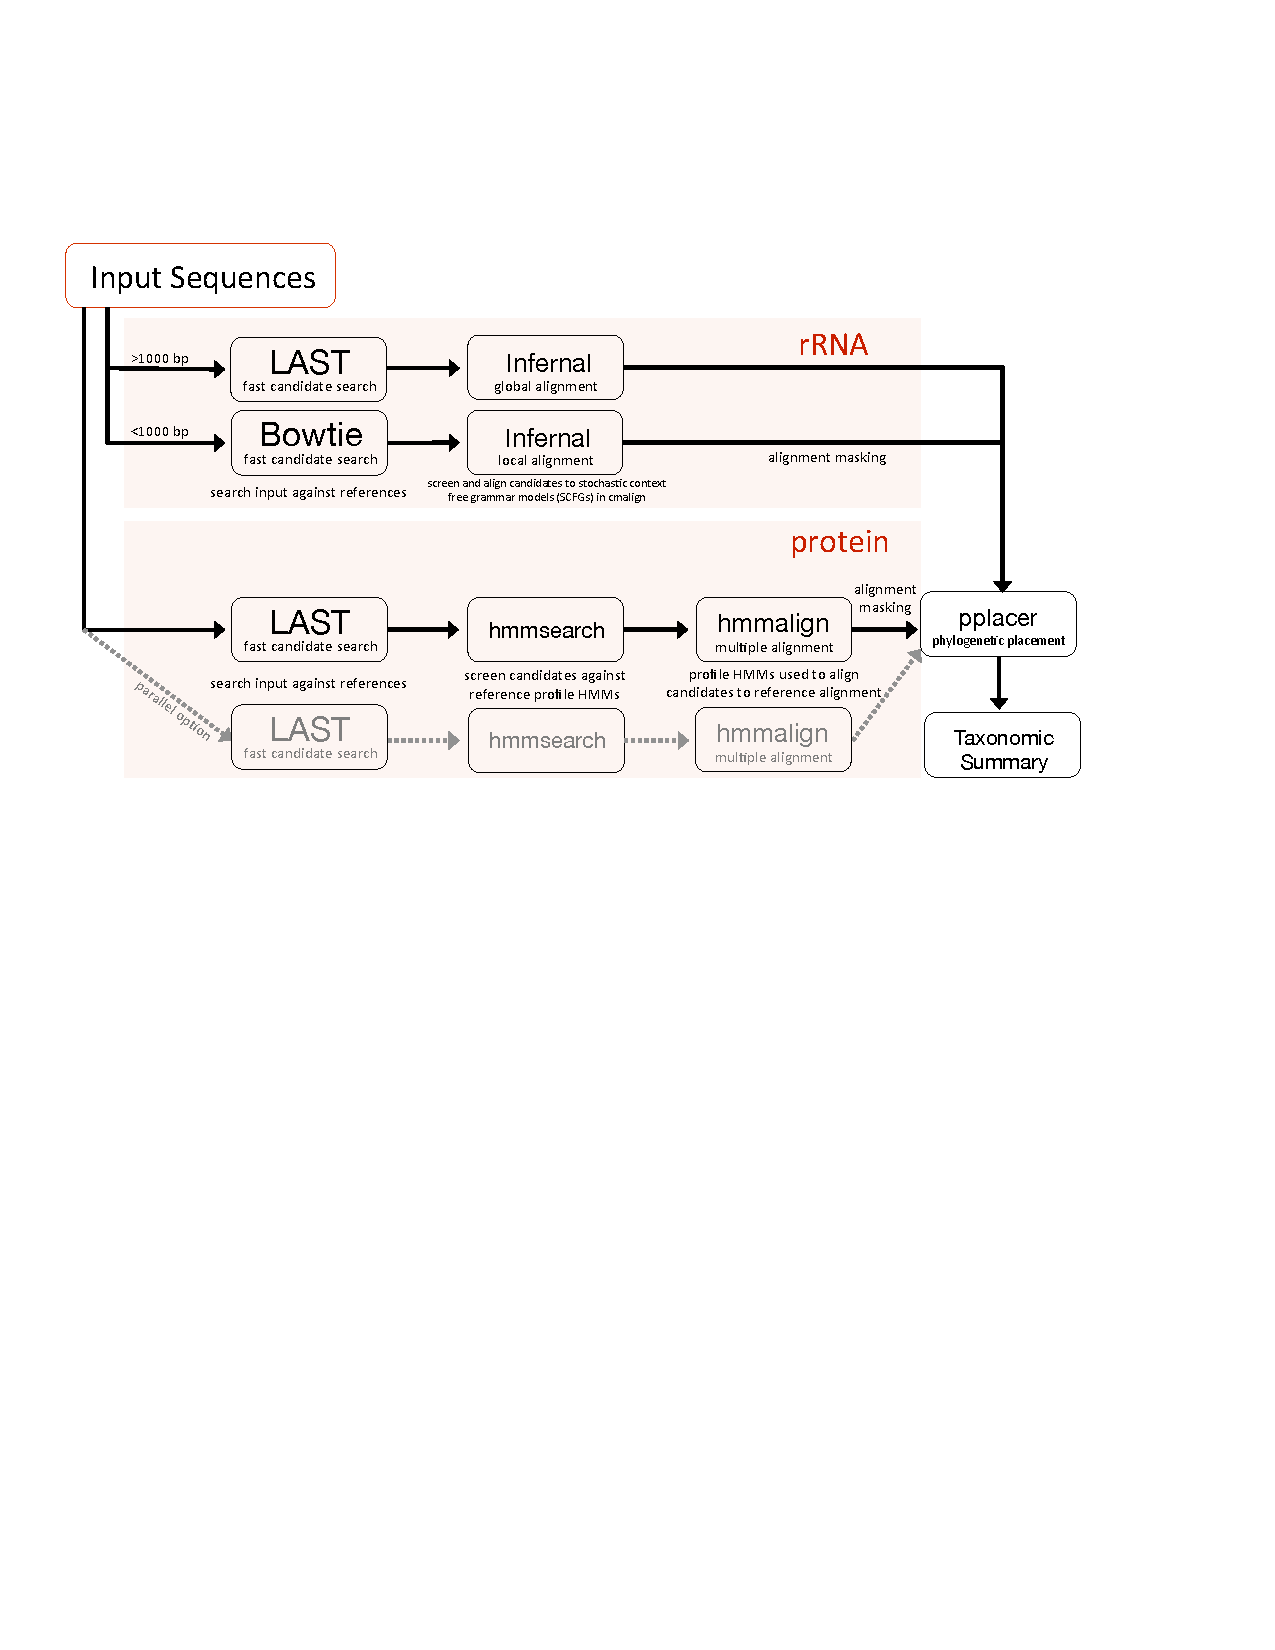
\includegraphics[trim=0 5.25in 0.5in 1.25in,clip,width=6.5in]{figures/Phylosift_overview_vector.pdf}
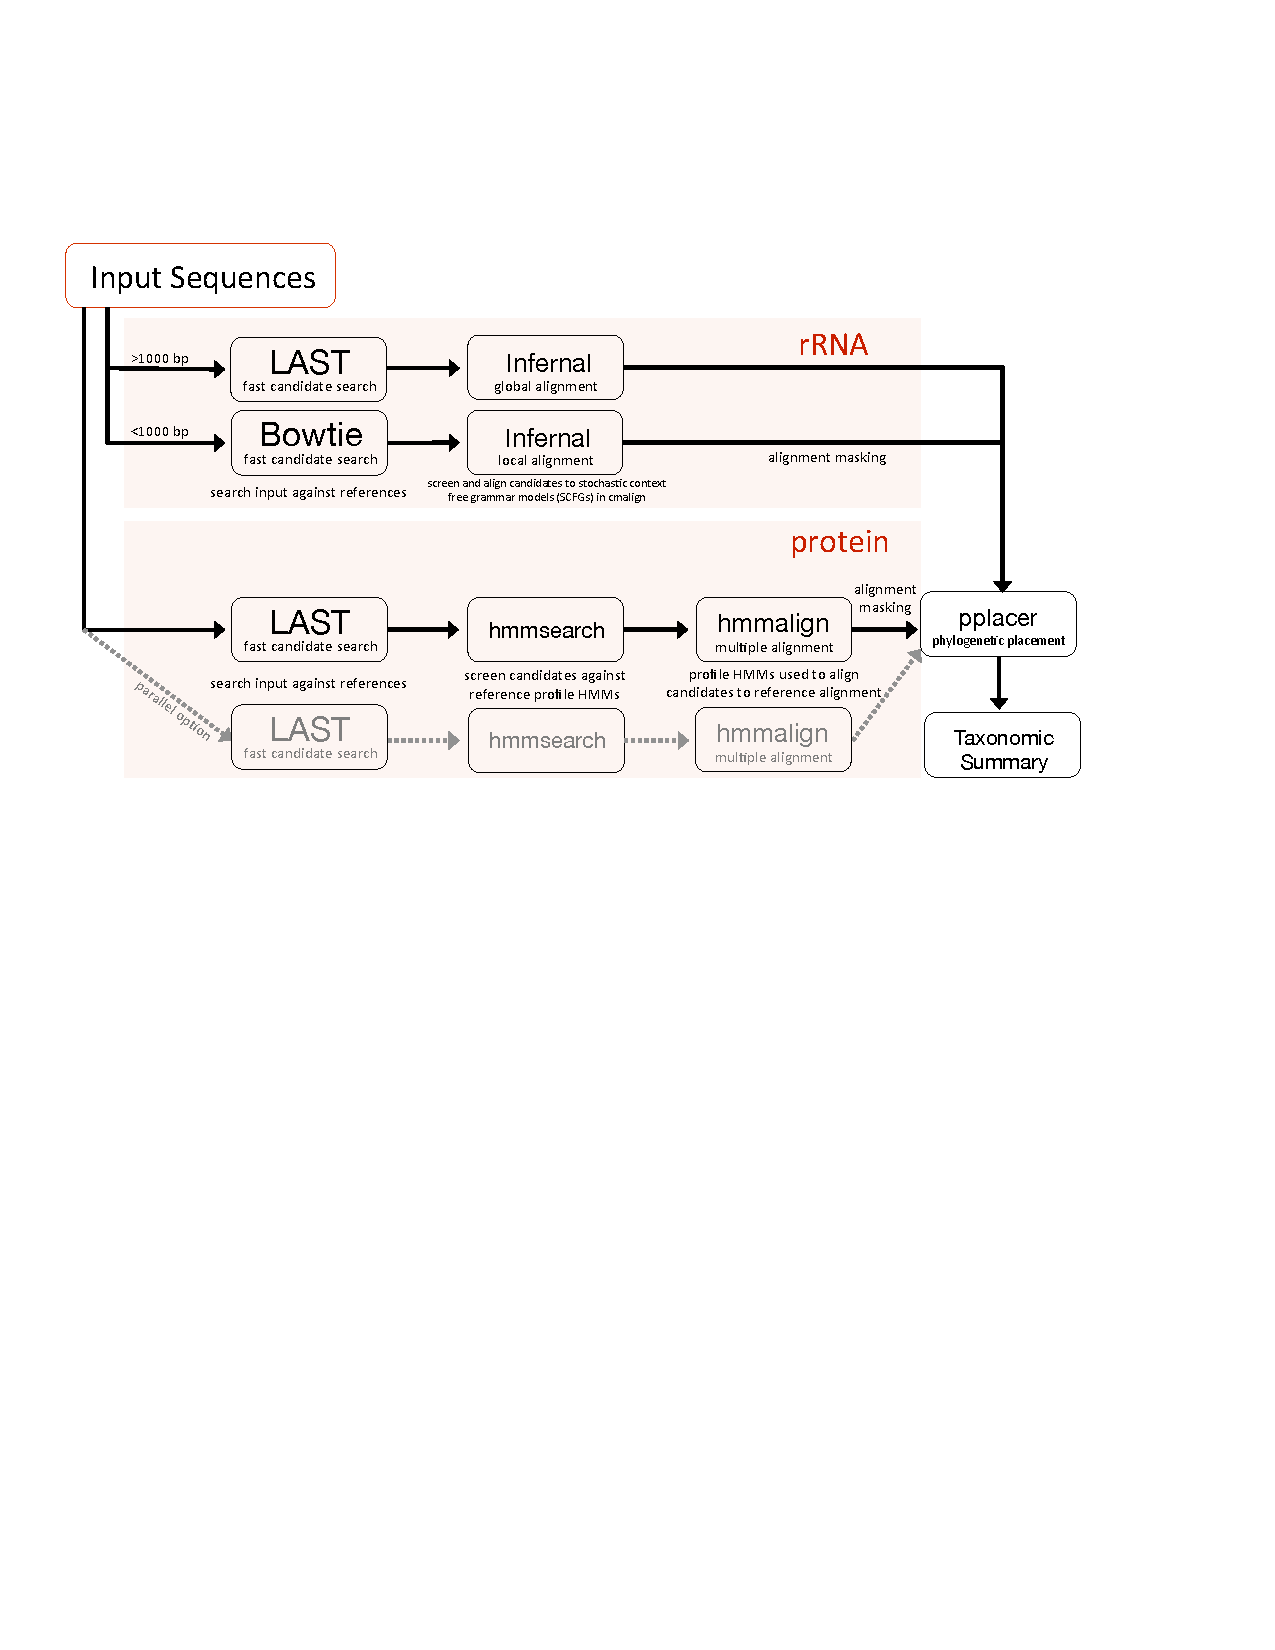
\includegraphics[width=6.5in]{figures/Phylosift_overview_vector.pdf}
\end{center}
\caption{\textbf{PhyloSift client workflow.} This workflow is applied to the user's sequence data.}
\label{fig:overview}
\end{figure}

\begin{figure}[hp]
\begin{center}
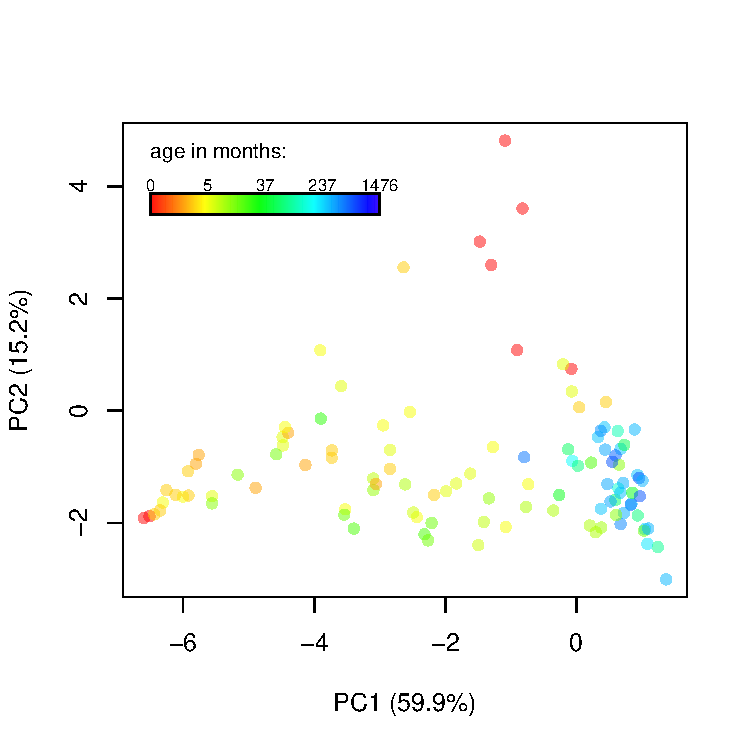
\includegraphics[width=4in]{figures/age_pca.pdf}
\end{center}
\caption{\textbf{Edge PCA analysis of human fecal samples.} 110 metagenomic samples were processed using PhyloSift and their community composition compared using Edge PCA.}
\label{fig:agepca}
\end{figure}

\begin{figure}[hp]
\begin{center}
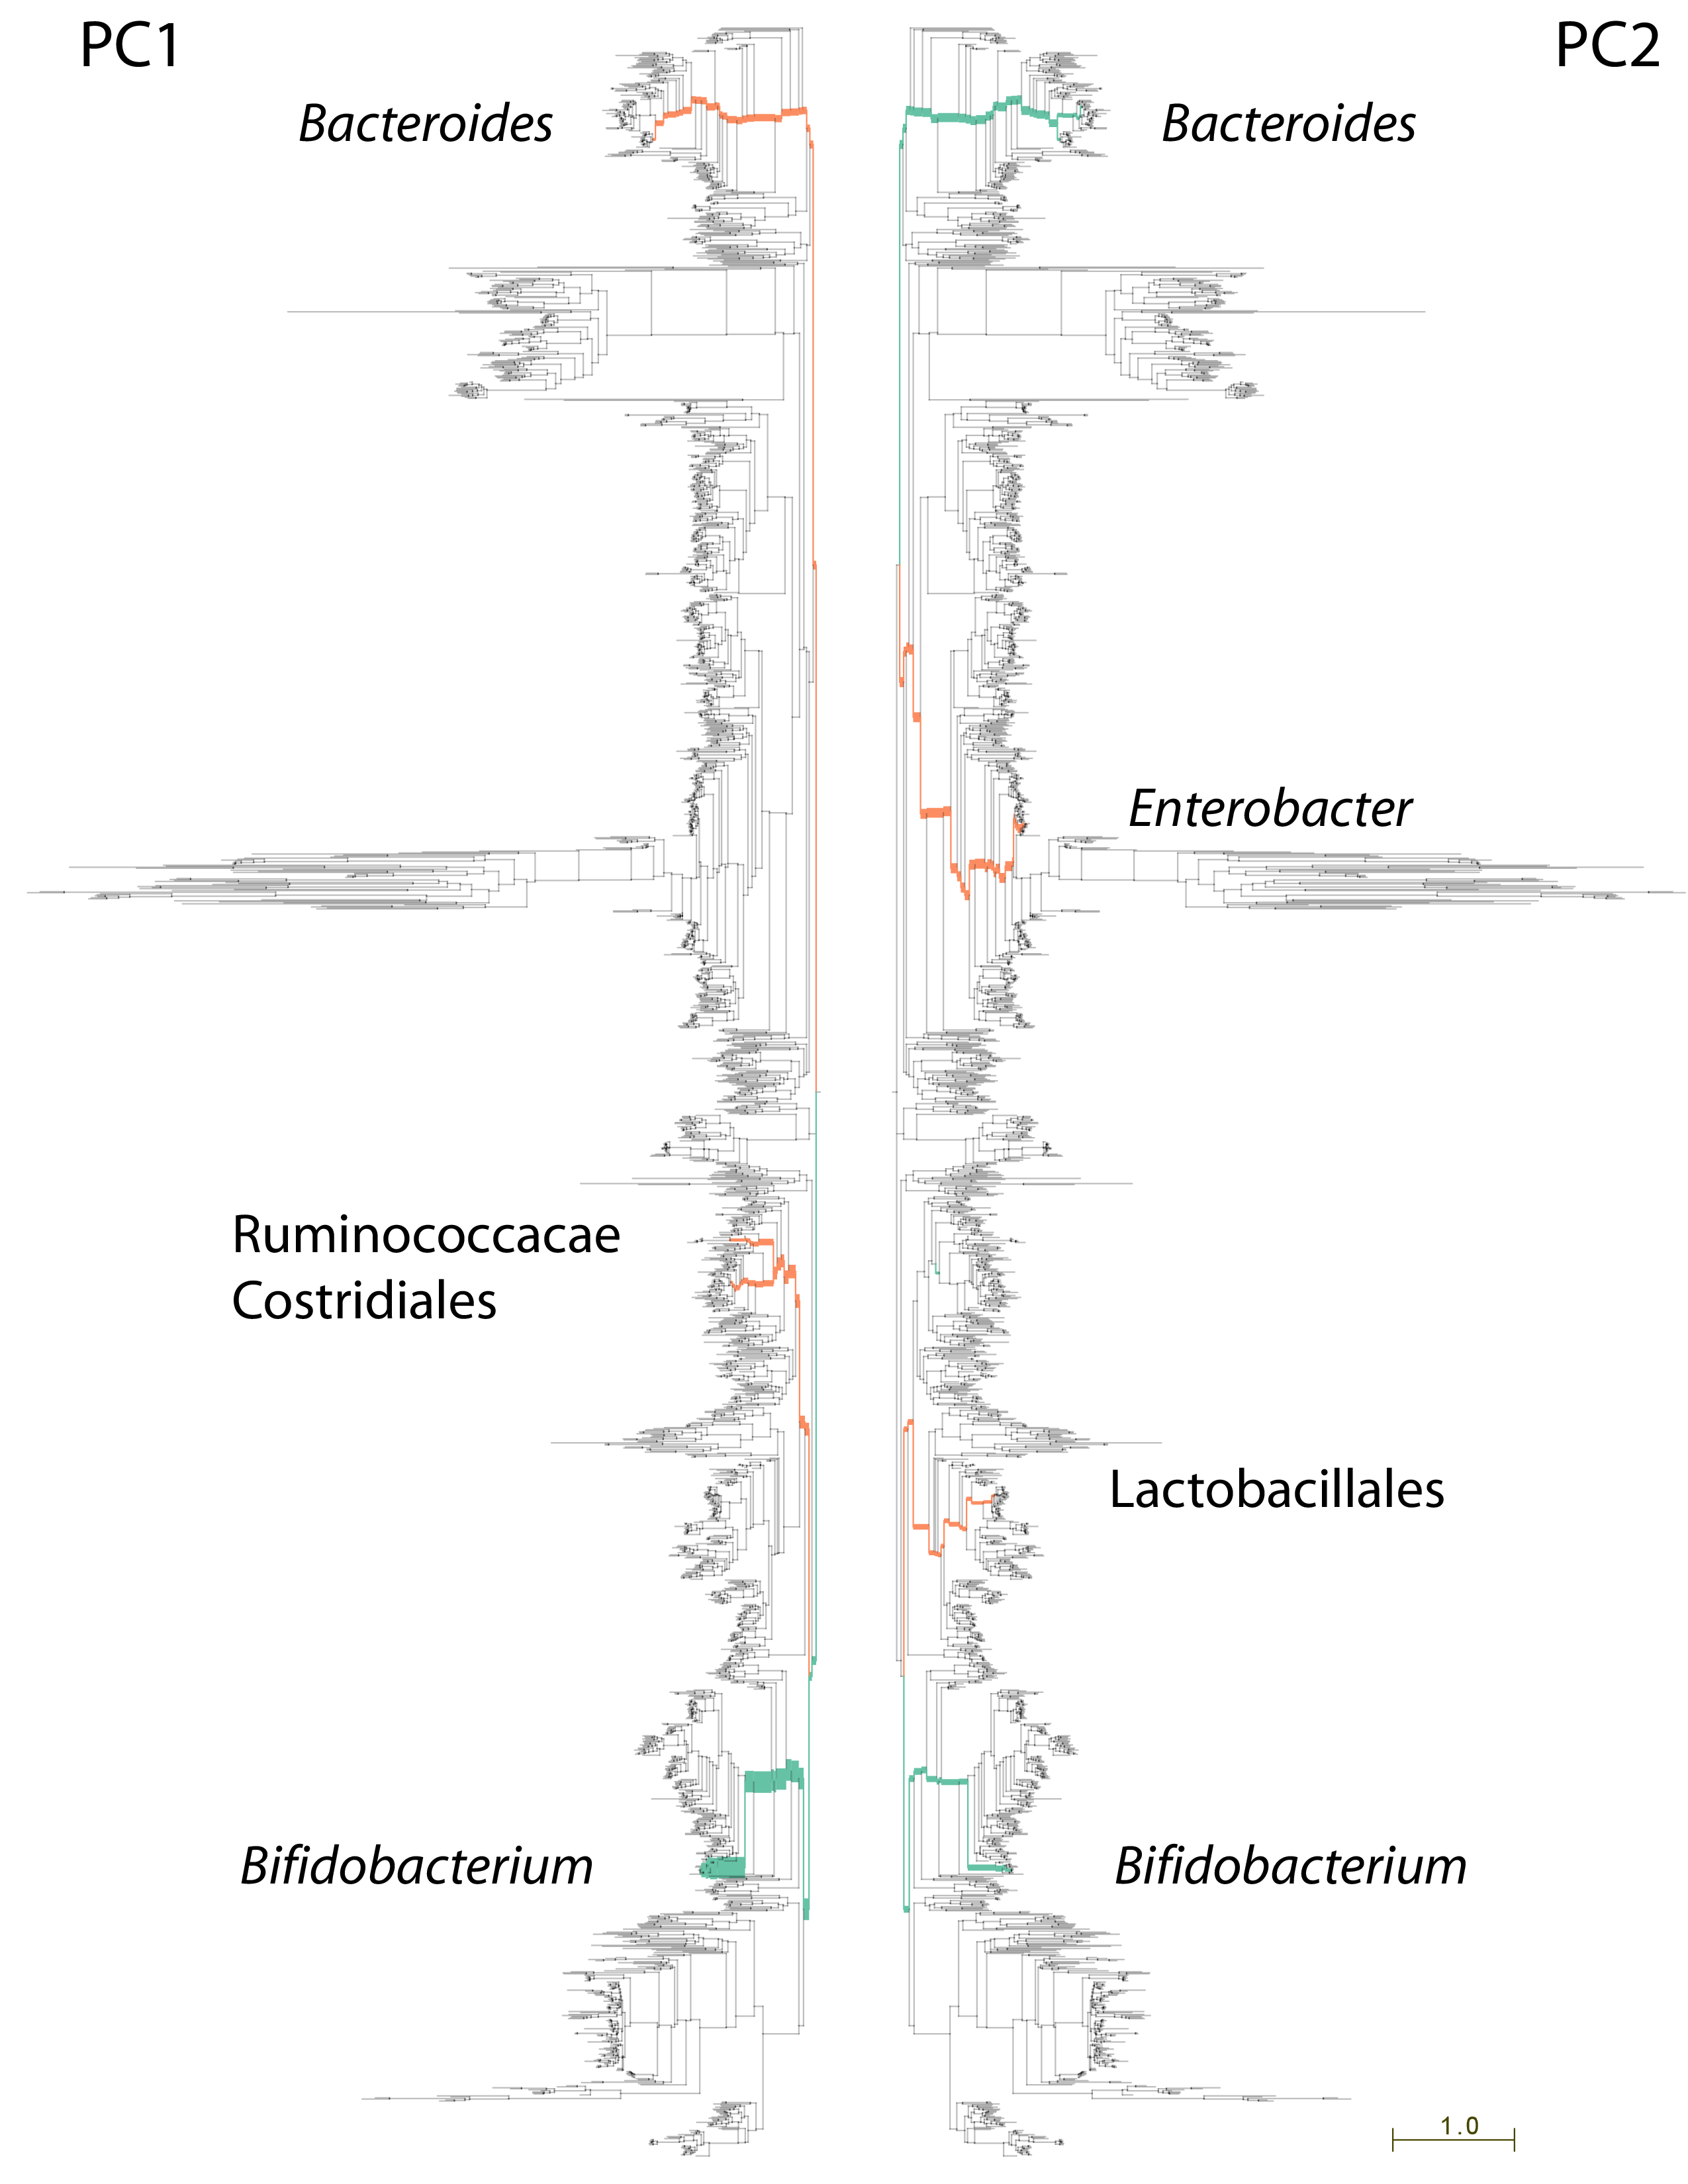
\includegraphics[width=6in]{figures/both_prettylike_b2b.pdf}
\end{center}
\caption{\textbf{Lineages contributing variation in human fecal sample community structure.} 110 metagenomic samples were processed using PhyloSift and their community composition compared using Edge PCA~\cite{Matsen2012}. Lineages that decrease in abundance along the principal component axis are shown in turquoise color, those increasing in abundance are shown in red. Edge width is proportional to the change in abundance. Remaining lineages in the phylogeny of bacteria, archaea, eukarya, and some viruses are shown in light gray. PC1 shown at left, PC2 at right.}
\label{fig:pcaphylo}
\end{figure}

\begin{figure}[hp]
\begin{center}
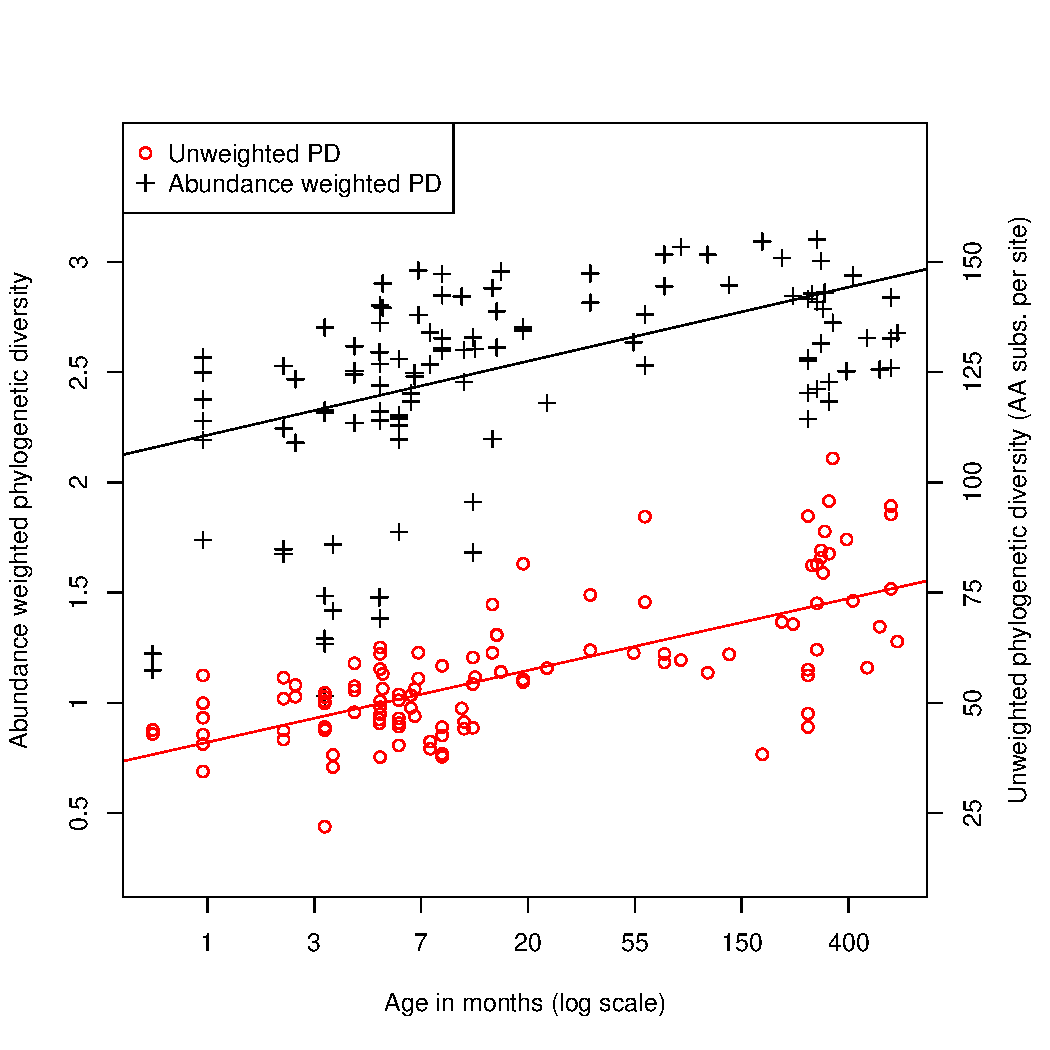
\includegraphics[width=4in]{figures/phylo_diversity.pdf}
\end{center}
\caption{\textbf{Relationship betwen fecal community phylogenetic diversity and host age.} 110 metagenomic samples were processed using PhyloSift and their phylogenetic diversity analyzed using two metrics. Unweighted phylogenetic diversity simply measures the total branch length of the reference tree covered by placed reads from a sample. Abundance-weighted phylogenetic diversity adjusts these values by the abundance of each lineage in the sample. In both cases, a log-linear relationship between host age and fecal community phylogenetic diversity can be observed.}
\label{fig:pcaphylo}
\end{figure}

\begin{figure}[hp]
\begin{center}
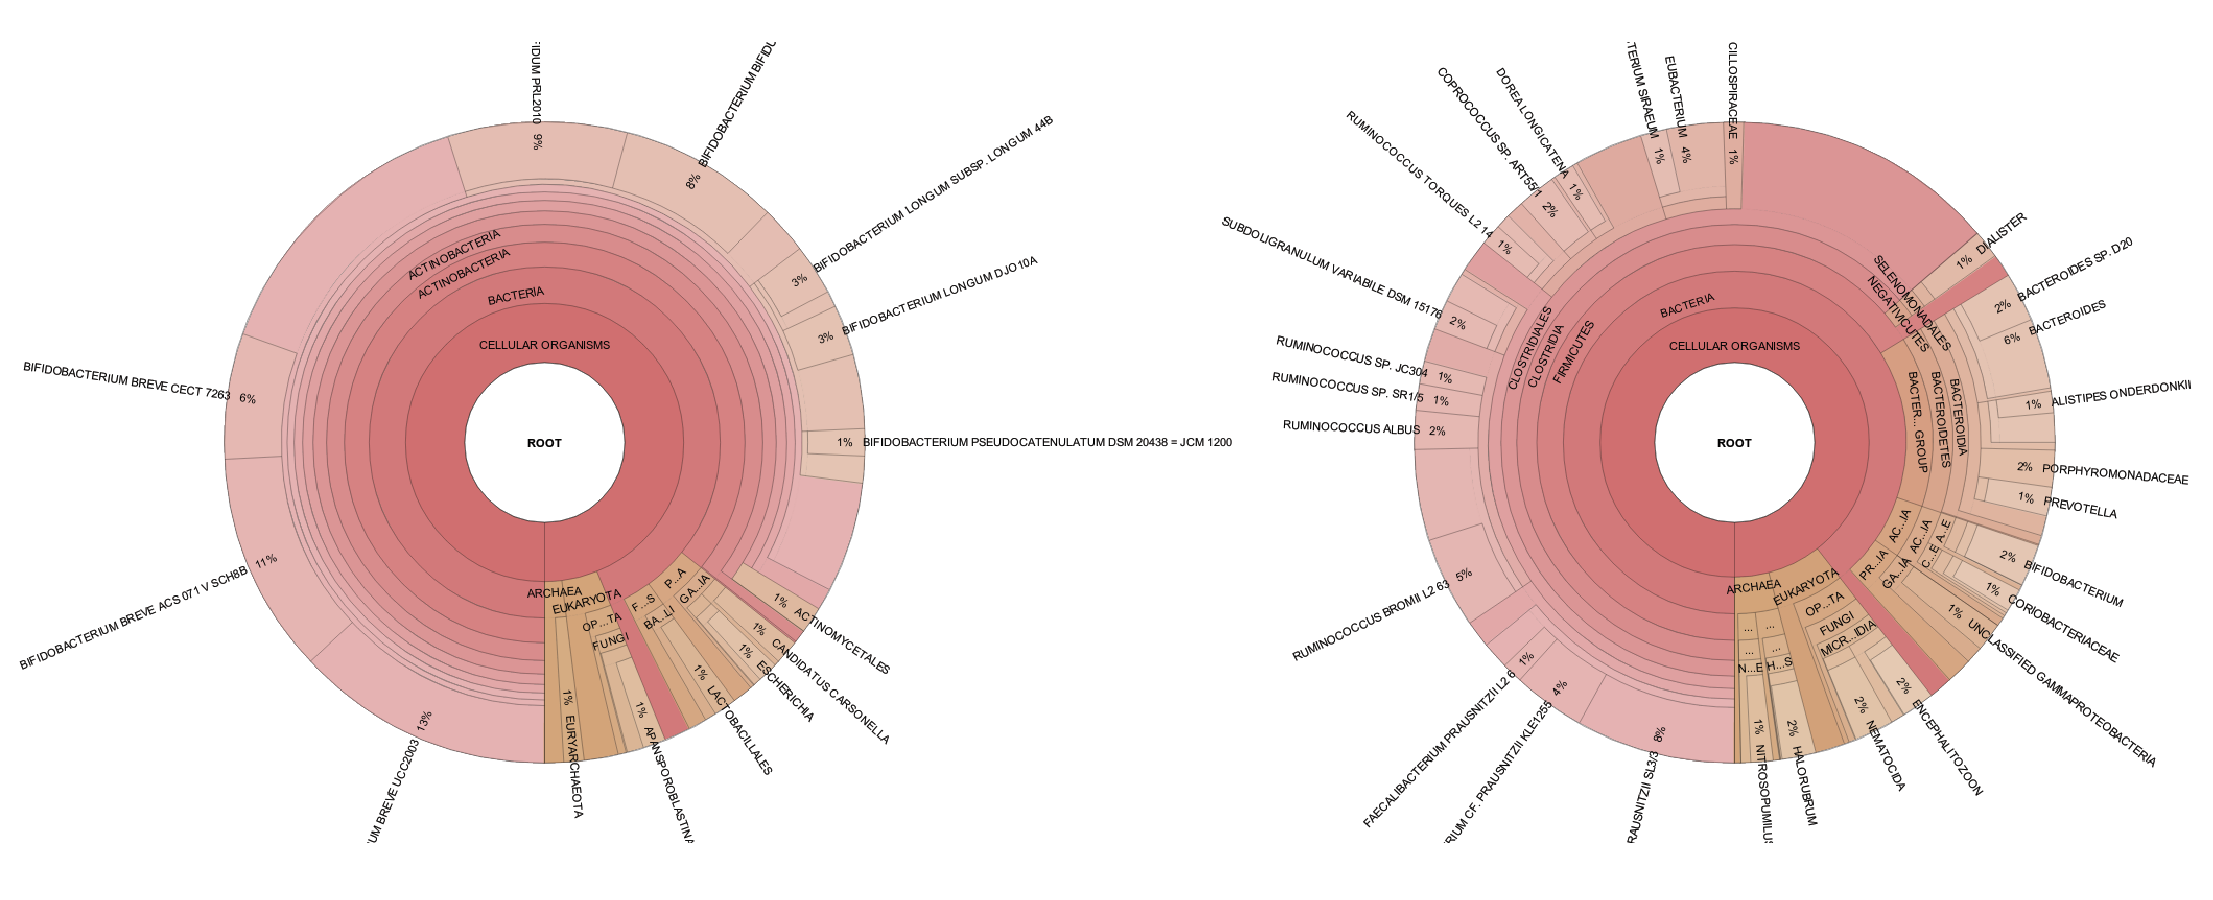
\includegraphics[width=6.5in]{figures/krona_two.pdf}
\end{center}
\caption{\textbf{Taxonomic visualization of two human gut samples.} Data analyzed by PhyloSift, visualized by Krona.}
\label{fig:kronaplots}
\end{figure}

\clearpage

\section*{Tables}


\clearpage

\end{document}

